%!TEX program = xelatex

% Name           : hsrm-beamer-demo.sty
% Author         : Benjamin Weiss (benjamin.weiss@kreatiefton.de)
% Version        : 0.4
% Created on     : 05.05.2013
% Last Edited on : 24.03.2014
% Copyright      : Copyright (c) 2013-2014 by Benjamin Weiss. All rights reserved.
% License        : This file may be distributed and/or modified under the
%                  GNU Public License.
% Description    : HSRM beamer theme demonstration. Also includes a short 
%                  Tutorial regarding the beamer class.

\documentclass[compress]{beamer}
%--------------------------------------------------------------------------
% Common packages
%--------------------------------------------------------------------------
\usepackage[german]{babel}

\usepackage{graphicx}
\usepackage{multicol}
% Erweiterte Tabellenfunktionen
\usepackage{tabularx,ragged2e}
\usepackage{booktabs}
% Listingserweiterung
\usepackage{listings}
\lstset{ %
language=[LaTeX]TeX,
basicstyle=\normalsize\ttfamily,
keywordstyle=,
numbers=left,
numberstyle=\tiny\ttfamily,
stepnumber=1,
showspaces=false,
showstringspaces=false,
showtabs=false,
breaklines=true,
frame=tb,
framerule=0.5pt,
tabsize=4,
framexleftmargin=0.5em,
framexrightmargin=0.5em,
xleftmargin=0.5em,
xrightmargin=0.5em
}

%--------------------------------------------------------------------------
% Load theme
%--------------------------------------------------------------------------
\usetheme{hsrm}

\usepackage{dtklogos} % must be loaded after theme
\usepackage{tikz}
\usetikzlibrary{mindmap,backgrounds}

%--------------------------------------------------------------------------
% General presentation settings
%--------------------------------------------------------------------------
\title{HSRM Beamer Theme}
\subtitle{Demonstration und kurze Einführung in Beamer}
\date{Letztes Update: \today}
\author{Benjamin Weiss}
\institute{Studienbereich Informations- und Elektrotechnik\\Hochschule {\Medium RheinMain}}

%--------------------------------------------------------------------------
% Notes settings
%--------------------------------------------------------------------------
\setbeameroption{show notes}

\begin{document}
%--------------------------------------------------------------------------
% Titlepage
%--------------------------------------------------------------------------

\maketitle

%\begin{frame}[plain]
%	\titlepage
%\end{frame}

%--------------------------------------------------------------------------
% Table of contents
%--------------------------------------------------------------------------
\section*{Gliederung}
\begin{frame}{Gliederung}
	% hideallsubsections ist empfehlenswert für längere Präsentationen
	\tableofcontents[hideallsubsections]
\end{frame}

%--------------------------------------------------------------------------
% Content
%--------------------------------------------------------------------------
\section{Einleitung}

\begin{frame}{Was ist Beamer?}
	Die Beamer Klassen für \LaTeX\ dienen zur Erstellung von Präsentationen, welche mit einem Beamer vorgeführt werden sollen. Das Textsatzsystem erzeugt dazu PDF Dateien, die von einer großen Anzahl an Programmen gezeigt werden können.
	
	Das hier vorgestellte Theme für Beamer macht die Erstellung von Folien entsprechend dem Corporate Design der Hochschule {\Medium RheinMain} (Grundkenntnisse in \LaTeX\ vorausgesetzt) zu einem Kinderspiel.
\end{frame}

\begin{frame}{Systemvoraussetzungen}
	Um erfolgreich Präsentationen mit diesem Theme erstellen zu können, sind folgende Voraussetzungen vom System zu erfüllen:
	\begin{itemize}
		\item Zum Setzen der Folien muss XeTeX verwendet werden.
		\item Neben einigen Standardpaketen müssen die Pakete \texttt{beamer}, \texttt{pgf} und \texttt{xcolor} installiert sein.
		\item Die Schriften \quoted{Flama-Light}, \quoted{Flama-Book} und \quoted{Flama-Medium} sollten installiert sein. Alternativ: \quoted{Arial}\\\url{http://www.felicianotypefoundry.com/}
	\end{itemize}
\end{frame}

\section{Tutorial}
\begin{frame}[containsverbatim]{Grundaufbau des Dokuments}
Der Grundaufbau ist einfach:
\begin{lstlisting}
\documentclass[compress]{beamer}
% Theme laden
\usetheme{hsrm}
% Allgemeine Präsentationseinstellungen 
\title{Titel der Präsentation}
\subtitle{Untertitel der Präsentation}
\author{Ihr Name}
\institute{Studienbereich\\Hochschule {\Medium RheinMain}}
\begin{document}
% Folien
\end{document}
\end{lstlisting}
\end{frame}

\begin{frame}{Themeoptionen}
Um die Darstellung der Präsentation anzupassen können die folgenden Optionen gewählt werden.
\begin{table}[]
	\begin{tabularx}{\linewidth}{l>{\raggedright}X}
		\toprule
		\textbf{Option}			& \textbf{Auswirkung} \tabularnewline
		\midrule
		\texttt{noflama}		& Falls Sie die Schrift Flama nicht besitzen können Sie mit dieser Option auf die Schrift Arial umschalten. \tabularnewline
		\texttt{noserifmath}		& Formeln werden ebenfalls serifenlos gesetzt. \tabularnewline
		\texttt{nosectionpages} & Die Sektionseinleitungsseiten werden ausgeblendet.\tabularnewline
		\bottomrule
	\end{tabularx}
	\label{tab:options}
\end{table}
\end{frame}

\begin{frame}{Primärfarben}									
Alle Farben des Corporate Designs sind im Template hinterlegt.


\begin{multicols}{2}

\setbeamercolor{hsrmRedDemo}{fg=hsrmRed,bg=white}
\begin{beamercolorbox}[wd=\linewidth,ht=2ex,dp=0.7ex]{hsrmRedDemo}
	\texttt{hsrmRed}
\end{beamercolorbox}
\setbeamercolor{hsrmRedDarkDemo}{fg=hsrmRedDark,bg=white}
\begin{beamercolorbox}[wd=\linewidth,ht=2ex,dp=0.7ex]{hsrmRedDarkDemo}
	\texttt{hsrmRedDark}
\end{beamercolorbox}
\setbeamercolor{hsrmWarmGreyDarkDemo}{fg=hsrmWarmGreyDark,bg=white}
\begin{beamercolorbox}[wd=\linewidth,ht=2ex,dp=0.7ex]{hsrmWarmGreyDarkDemo}
	\texttt{hsrmWarmGreyDark}
\end{beamercolorbox}
\setbeamercolor{hsrmWarmGreyLightDemo}{fg=hsrmWarmGreyLight,bg=white}
\begin{beamercolorbox}[wd=\linewidth,ht=2ex,dp=0.7ex]{hsrmWarmGreyLightDemo}
	\texttt{hsrmWarmGreyLight}
\end{beamercolorbox}

\setbeamercolor{hsrmRedDemoBg}{fg=white,bg=hsrmRed}
\begin{beamercolorbox}[wd=\linewidth,ht=2ex,leftskip=.5ex,dp=0.7ex]{hsrmRedDemoBg}
	\texttt{hsrmRed}
\end{beamercolorbox}
\setbeamercolor{hsrmRedDarkDemoBg}{fg=white,bg=hsrmRedDark}
\begin{beamercolorbox}[wd=\linewidth,ht=2ex,leftskip=.5ex,dp=0.7ex]{hsrmRedDarkDemoBg}
	\texttt{hsrmRedDark}
\end{beamercolorbox}
\setbeamercolor{hsrmWarmGreyDarkDemo}{fg=white,bg=hsrmWarmGreyDark}
\begin{beamercolorbox}[wd=\linewidth,ht=2ex,leftskip=.5ex,dp=0.7ex]{hsrmWarmGreyDarkDemo}
	\texttt{hsrmWarmGreyDark}
\end{beamercolorbox}
\setbeamercolor{hsrmWarmGreyLightDemo}{fg=white,bg=hsrmWarmGreyLight}
\begin{beamercolorbox}[wd=\linewidth,ht=2ex,leftskip=.5ex,dp=0.7ex]{hsrmWarmGreyLightDemo}
	\texttt{hsrmWarmGreyLight}
\end{beamercolorbox}

\end{multicols}

\end{frame}

\begin{frame}{Sekundärfarben}
\begin{multicols}{2}

\setbeamercolor{hsrmSec1Demo}{fg=hsrmSec1,bg=white}
\begin{beamercolorbox}[wd=\linewidth,ht=2ex,dp=0.7ex]{hsrmSec1Demo}
	\texttt{hsrmSec1}
\end{beamercolorbox}
\setbeamercolor{hsrmSec1DarkDemo}{fg=hsrmSec1Dark,bg=white}
\begin{beamercolorbox}[wd=\linewidth,ht=2ex,dp=0.7ex]{hsrmSec1DarkDemo}
	\texttt{hsrmSec1Dark}
\end{beamercolorbox}
\setbeamercolor{hsrmSec1CompDemo}{fg=hsrmSec1Comp,bg=white}
\begin{beamercolorbox}[wd=\linewidth,ht=2ex,dp=0.7ex]{hsrmSec1CompDemo}
	\texttt{hsrmSec1Comp}
\end{beamercolorbox}
\setbeamercolor{hsrmSec1CompDarkDemo}{fg=hsrmSec1CompDark,bg=white}
\begin{beamercolorbox}[wd=\linewidth,ht=2ex,dp=0.7ex]{hsrmSec1CompDarkDemo}
	\texttt{hsrmSec1CompDark}
\end{beamercolorbox}

\setbeamercolor{hsrmSec2Demo}{fg=hsrmSec2,bg=white}
\begin{beamercolorbox}[wd=\linewidth,ht=2ex,dp=0.7ex]{hsrmSec2Demo}
	\texttt{hsrmSec2}
\end{beamercolorbox}
\setbeamercolor{hsrmSec2DarkDemo}{fg=hsrmSec2Dark,bg=white}
\begin{beamercolorbox}[wd=\linewidth,ht=2ex,dp=0.7ex]{hsrmSec2DarkDemo}
	\texttt{hsrmSec2Dark}
\end{beamercolorbox}
\setbeamercolor{hsrmSec2CompDemo}{fg=hsrmSec2Comp,bg=white}
\begin{beamercolorbox}[wd=\linewidth,ht=2ex,dp=0.7ex]{hsrmSec2CompDemo}
	\texttt{hsrmSec2Comp}
\end{beamercolorbox}
\setbeamercolor{hsrmSec2CompDarkDemo}{fg=hsrmSec2CompDark,bg=white}
\begin{beamercolorbox}[wd=\linewidth,ht=2ex,dp=0.7ex]{hsrmSec2CompDarkDemo}
	\texttt{hsrmSec2CompDark}
\end{beamercolorbox}

\setbeamercolor{hsrmSec3Demo}{fg=hsrmSec3,bg=white}
\begin{beamercolorbox}[wd=\linewidth,ht=2ex,dp=0.7ex]{hsrmSec3Demo}
	\texttt{hsrmSec3}
\end{beamercolorbox}
\setbeamercolor{hsrmSec3DarkDemo}{fg=hsrmSec3Dark,bg=white}
\begin{beamercolorbox}[wd=\linewidth,ht=2ex,dp=0.7ex]{hsrmSec3DarkDemo}
	\texttt{hsrmSec3Dark}
\end{beamercolorbox}
\setbeamercolor{hsrmSec3CompDemo}{fg=hsrmSec3Comp,bg=white}
\begin{beamercolorbox}[wd=\linewidth,ht=2ex,dp=0.7ex]{hsrmSec3CompDemo}
	\texttt{hsrmSec3Comp}
\end{beamercolorbox}
\setbeamercolor{hsrmSec3CompDarkDemo}{fg=hsrmSec3CompDark,bg=white}
\begin{beamercolorbox}[wd=\linewidth,ht=2ex,dp=0.7ex]{hsrmSec3CompDarkDemo}
	\texttt{hsrmSec3CompDark}
\end{beamercolorbox}

\setbeamercolor{hsrmSec1DemoBg}{fg=white,bg=hsrmSec1}
\begin{beamercolorbox}[wd=\linewidth,ht=2ex,leftskip=.5ex,dp=0.7ex]{hsrmSec1DemoBg}
	\texttt{hsrmSec1}
\end{beamercolorbox}
\setbeamercolor{hsrmSec1DarkDemoBg}{fg=white,bg=hsrmSec1Dark}
\begin{beamercolorbox}[wd=\linewidth,ht=2ex,leftskip=.5ex,dp=0.7ex]{hsrmSec1DarkDemoBg}
	\texttt{hsrmSec1Dark}
\end{beamercolorbox}
\setbeamercolor{hsrmSec1CompDemoBg}{fg=white,bg=hsrmSec1Comp}
\begin{beamercolorbox}[wd=\linewidth,ht=2ex,leftskip=.5ex,dp=0.7ex]{hsrmSec1CompDemoBg}
	\texttt{hsrmSec1Comp}
\end{beamercolorbox}
\setbeamercolor{hsrmSec1CompDarkDemoBg}{fg=white,bg=hsrmSec1CompDark}
\begin{beamercolorbox}[wd=\linewidth,ht=2ex,leftskip=.5ex,dp=0.7ex]{hsrmSec1CompDarkDemoBg}
	\texttt{hsrmSec1CompDark}
\end{beamercolorbox}

\setbeamercolor{hsrmSec2DemoBg}{fg=white,bg=hsrmSec2}
\begin{beamercolorbox}[wd=\linewidth,ht=2ex,leftskip=.5ex,dp=0.7ex]{hsrmSec2DemoBg}
	\texttt{hsrmSec2}
\end{beamercolorbox}
\setbeamercolor{hsrmSec2DarkDemoBg}{fg=white,bg=hsrmSec2Dark}
\begin{beamercolorbox}[wd=\linewidth,ht=2ex,leftskip=.5ex,dp=0.7ex]{hsrmSec2DarkDemoBg}
	\texttt{hsrmSec2Dark}
\end{beamercolorbox}
\setbeamercolor{hsrmSec2CompDemoBg}{fg=white,bg=hsrmSec2Comp}
\begin{beamercolorbox}[wd=\linewidth,ht=2ex,leftskip=.5ex,dp=0.7ex]{hsrmSec2CompDemoBg}
	\texttt{hsrmSec2Comp}
\end{beamercolorbox}
\setbeamercolor{hsrmSec2CompDarkDemoBg}{fg=white,bg=hsrmSec2CompDark}
\begin{beamercolorbox}[wd=\linewidth,ht=2ex,leftskip=.5ex,dp=0.7ex]{hsrmSec2CompDarkDemoBg}
	\texttt{hsrmSec2CompDark}
\end{beamercolorbox}

\setbeamercolor{hsrmSec3Demo}{fg=white,bg=hsrmSec3}
\begin{beamercolorbox}[wd=\linewidth,ht=2ex,leftskip=.5ex,dp=0.7ex]{hsrmSec3Demo}
	\texttt{hsrmSec3}
\end{beamercolorbox}
\setbeamercolor{hsrmSec3DarkDemo}{fg=white,bg=hsrmSec3Dark}
\begin{beamercolorbox}[wd=\linewidth,ht=2ex,leftskip=.5ex,dp=0.7ex]{hsrmSec3DarkDemo}
	\texttt{hsrmSec3Dark}
\end{beamercolorbox}
\setbeamercolor{hsrmSec3CompDemo}{fg=white,bg=hsrmSec3Comp}
\begin{beamercolorbox}[wd=\linewidth,ht=2ex,leftskip=.5ex,dp=0.7ex]{hsrmSec3CompDemo}
	\texttt{hsrmSec3Comp}
\end{beamercolorbox}
\setbeamercolor{hsrmSec3CompDarkDemo}{fg=white,bg=hsrmSec3CompDark}
\begin{beamercolorbox}[wd=\linewidth,ht=2ex,leftskip=.5ex,dp=0.7ex]{hsrmSec3CompDarkDemo}
	\texttt{hsrmSec3CompDark}
\end{beamercolorbox}

\end{multicols}
\end{frame}

\begin{frame}[containsverbatim]{Folienstruktur}
Strukturiert wird in Beamer wie in \LaTeX\ üblich mittels \lstinline!section!, \lstinline!subsection!, usw. Für Folien ist die \lstinline!frame! Umgebung definiert.

Der Folientitel kann direkt an die \lstinline!frame! Umgebung übergeben werden oder mittels \lstinline!\frametitle{Folientitel}! innerhalb der Umgebung gesetzt werden.
\begin{lstlisting}
\section{Meine Sektion}
\subsection{Meine Subsektion}
\begin{frame}
\frametitle{Folientitel}
% Folieninhalt
\end{frame}
\end{lstlisting}
\end{frame}

\begin{frame}[containsverbatim]{Titelseite und Inhaltsverzeichnis}
Die Titelseite erzeugt man mit 
\begin{lstlisting}
\maketitle
\end{lstlisting}
Und das Inhaltsverzeichnis mit
\begin{lstlisting}
\begin{frame}{Gliederung}
	\tableofcontents[hideallsubsections]
\end{frame}
\end{lstlisting}
Die Option \lstinline!hideallsubsections! bietet sich bei längeren Präsentationen an, um das Inhaltsverzeichnis kompakt zu halten.
\end{frame}

\subsection{Aufzählungen}
\begin{frame}[containsverbatim]{Aufzählungen}
Aufzählungen sind mit der \lstinline!enumerate! und der \lstinline!itemize! Umgebung möglich.
\begin{enumerate}
	\item Punkt 1
	\item Punkt 2
	\begin{itemize}
		\item Punkt 1
		\item Punkt 2
	\end{itemize}
	\item Punkt 3
\end{enumerate}
\end{frame}

\subsection{Hervorhebungen}
\begin{frame}[containsverbatim]{Hervorhebungen}
In der Beamer Klasse ist die Funktion \lstinline!\alert! definiert, um einzelne Wörter hervorzuheben. Beispiel:
\begin{itemize}
	\item \alert{hervorgehobener Text}
\end{itemize}
Zusätzlich sind im HSRM Theme noch \lstinline!\quoted! und \lstinline!\doublequoted! definiert, um die Anführungszeichen des Corporate Designs der Hochschule einfach im Zugriff zu haben. Beispiele:
\begin{itemize}
	\item[] \quoted{Einfache Anführungszeichen}
	\item[] \doublequoted{Doppelte Anführungszeichen}
\end{itemize}
\end{frame}

\subsection{Blockstrukturen}
\begin{frame}[containsverbatim]{Einfacher Block mit Aufzählung}
Zur Strukturierung sind in Beamer Blockumgebungen definiert.
\begin{block}{Block mit einer Aufzählung}
	\begin{itemize}
		\item Punkt 1
		\item Punkt 2
	\end{itemize}
\end{block}
\begin{lstlisting}
\begin{block}{Block mit einer Aufzählung}
	\begin{itemize}
		\item Punkt 1
		\item Punkt 2
	\end{itemize}
\end{block}
\end{lstlisting}
\end{frame}

\begin{frame}[containsverbatim]{Alert Block}
\begin{alertblock}{Alert Block}
	Ein Alert Block wird mit der ersten Primärfarbe eingefärbt.
\end{alertblock}
\begin{lstlisting}
\begin{alertblock}{Alert Block}
Ein Alert Block wird mit der ersten Primärfarbe eingefärbt.
\end{alertblock}
\end{lstlisting}
\end{frame}

\begin{frame}[containsverbatim]{Example Block}
\begin{exampleblock}{Example Block}
	Ein Example Block wird mit der ersten Sekundärfarbe eingefärbt.
\end{exampleblock}
\begin{lstlisting}
\begin{exampleblock}{Example Block}
Ein Example Block wird mit der ersten Sekundärfarbe eingefärbt.
\end{exampleblock}
\end{lstlisting}
\end{frame}

\begin{frame}[containsverbatim]{Block mit anderer Farbe}
\begingroup
\setbeamercolor{block title}{bg=hsrmSec2Dark}
\setbeamercolor{block body}{bg=hsrmSec2}
\begin{block}{Block mit anderer Farbe}
	In diesem Block wird eine weitere Sekundärfarbe verwendet.
\end{block}
\endgroup
\begin{lstlisting}
\begingroup
\setbeamercolor{block title}{bg=hsrmSec2Dark}
\setbeamercolor{block body}{bg=hsrmSec2}
\begin{block}{Block mit anderer Farbe}
	In diesem Block wird ...
\end{block}
\endgroup
\end{lstlisting}
\end{frame}

\section{Beispielfolien}
\begin{frame}{Weitere Beispiele}
Nachfolgend sind weitere Beispielfolien ohne zusätzliche Erläuterung angehängt.

Schauen Sie einfach in den Quelltext, um zu sehen wie die Folien erstellt wurden.
\end{frame}
\subsection{Abbildungen}
\begin{frame}{Foto mit Copyright}
	\begin{figure}
		\centering
		\includegraphicscopyright[width=\linewidth]{photo.jpg}{Copyright by \href{http://netzlemming.deviantart.com/}{Netzlemming}, \href{http://creativecommons.org/licenses/by-nc/3.0/}{CC BY-NC 3.0 License}}
	\end{figure}
\end{frame}
\begin{frame}{Plot mit Beschriftung}
	\begin{figure}
		\centering
		% GNUPLOT: LaTeX picture with Postscript
\begingroup
  \makeatletter
  \providecommand\color[2][]{%
    \GenericError{(gnuplot) \space\space\space\@spaces}{%
      Package color not loaded in conjunction with
      terminal option `colourtext'%
    }{See the gnuplot documentation for explanation.%
    }{Either use 'blacktext' in gnuplot or load the package
      color.sty in LaTeX.}%
    \renewcommand\color[2][]{}%
  }%
  \providecommand\includegraphics[2][]{%
    \GenericError{(gnuplot) \space\space\space\@spaces}{%
      Package graphicx or graphics not loaded%
    }{See the gnuplot documentation for explanation.%
    }{The gnuplot epslatex terminal needs graphicx.sty or graphics.sty.}%
    \renewcommand\includegraphics[2][]{}%
  }%
  \providecommand\rotatebox[2]{#2}%
  \@ifundefined{ifGPcolor}{%
    \newif\ifGPcolor
    \GPcolorfalse
  }{}%
  \@ifundefined{ifGPblacktext}{%
    \newif\ifGPblacktext
    \GPblacktexttrue
  }{}%
  % define a \g@addto@macro without @ in the name:
  \let\gplgaddtomacro\g@addto@macro
  % define empty templates for all commands taking text:
  \gdef\gplbacktext{}%
  \gdef\gplfronttext{}%
  \makeatother
  \ifGPblacktext
    % no textcolor at all
    \def\colorrgb#1{}%
    \def\colorgray#1{}%
  \else
    % gray or color?
    \ifGPcolor
      \def\colorrgb#1{\color[rgb]{#1}}%
      \def\colorgray#1{\color[gray]{#1}}%
      \expandafter\def\csname LTw\endcsname{\color{white}}%
      \expandafter\def\csname LTb\endcsname{\color{black}}%
      \expandafter\def\csname LTa\endcsname{\color{black}}%
      \expandafter\def\csname LT0\endcsname{\color[rgb]{1,0,0}}%
      \expandafter\def\csname LT1\endcsname{\color[rgb]{0,1,0}}%
      \expandafter\def\csname LT2\endcsname{\color[rgb]{0,0,1}}%
      \expandafter\def\csname LT3\endcsname{\color[rgb]{1,0,1}}%
      \expandafter\def\csname LT4\endcsname{\color[rgb]{0,1,1}}%
      \expandafter\def\csname LT5\endcsname{\color[rgb]{1,1,0}}%
      \expandafter\def\csname LT6\endcsname{\color[rgb]{0,0,0}}%
      \expandafter\def\csname LT7\endcsname{\color[rgb]{1,0.3,0}}%
      \expandafter\def\csname LT8\endcsname{\color[rgb]{0.5,0.5,0.5}}%
    \else
      % gray
      \def\colorrgb#1{\color{black}}%
      \def\colorgray#1{\color[gray]{#1}}%
      \expandafter\def\csname LTw\endcsname{\color{white}}%
      \expandafter\def\csname LTb\endcsname{\color{black}}%
      \expandafter\def\csname LTa\endcsname{\color{black}}%
      \expandafter\def\csname LT0\endcsname{\color{black}}%
      \expandafter\def\csname LT1\endcsname{\color{black}}%
      \expandafter\def\csname LT2\endcsname{\color{black}}%
      \expandafter\def\csname LT3\endcsname{\color{black}}%
      \expandafter\def\csname LT4\endcsname{\color{black}}%
      \expandafter\def\csname LT5\endcsname{\color{black}}%
      \expandafter\def\csname LT6\endcsname{\color{black}}%
      \expandafter\def\csname LT7\endcsname{\color{black}}%
      \expandafter\def\csname LT8\endcsname{\color{black}}%
    \fi
  \fi
  \setlength{\unitlength}{0.0500bp}%
  \begin{picture}(4534.00,3400.00)%
    \gplgaddtomacro\gplbacktext{%
      \csname LTb\endcsname%
      \put(946,772){\makebox(0,0)[r]{\strut{}-140}}%
      \csname LTb\endcsname%
      \put(946,1109){\makebox(0,0)[r]{\strut{}-120}}%
      \csname LTb\endcsname%
      \put(946,1447){\makebox(0,0)[r]{\strut{}-100}}%
      \csname LTb\endcsname%
      \put(946,1784){\makebox(0,0)[r]{\strut{}-80}}%
      \csname LTb\endcsname%
      \put(946,2122){\makebox(0,0)[r]{\strut{}-60}}%
      \csname LTb\endcsname%
      \put(946,2460){\makebox(0,0)[r]{\strut{}-40}}%
      \csname LTb\endcsname%
      \put(946,2797){\makebox(0,0)[r]{\strut{}-20}}%
      \csname LTb\endcsname%
      \put(946,3135){\makebox(0,0)[r]{\strut{} 0}}%
      \csname LTb\endcsname%
      \put(1772,484){\makebox(0,0){\strut{} 100}}%
      \csname LTb\endcsname%
      \put(2766,484){\makebox(0,0){\strut{} 1000}}%
      \csname LTb\endcsname%
      \put(3759,484){\makebox(0,0){\strut{} 10000}}%
      \csname LTb\endcsname%
      \put(176,1919){\rotatebox{-270}{\makebox(0,0){\strut{}amplitude (dB)}}}%
      \put(2607,154){\makebox(0,0){\strut{}frequency (Hz)}}%
    }%
    \gplgaddtomacro\gplfronttext{%
    }%
    \gplbacktext
    \put(0,0){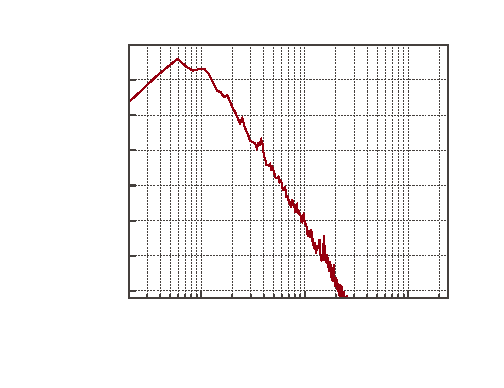
\includegraphics{plot}}%
    \gplfronttext
  \end{picture}%
\endgroup

		\caption{LFE channel frequency spectrum}
	\end{figure}
\end{frame}

\subsection{Tabellen}
\begin{frame}{Tabelle}
\begin{table}[]
	\caption{Selection of window function and their properties}
	\begin{tabular}[]{lrrr}
		\toprule
		\textbf{Window}			& \multicolumn{1}{c}{\textbf{First side lobe}}	
		                    & \multicolumn{1}{c}{\textbf{3\,dB bandwidth}}
		                    & \multicolumn{1}{c}{\textbf{Roll-off}} \\
		\midrule
		Rectangular				& 13.2\,dB	& 0.886\,Hz/bin	& 6\,dB/oct		\\[0.25em]
		Triangular				& 26.4\,dB	& 1.276\,Hz/bin	& 12\,dB/oct	\\[0.25em]
		Hann					& 31.0\,dB	& 1.442\,Hz/bin	& 18\,dB/oct	\\[0.25em]
		Hamming					& 41.0\,dB	& 1.300\,Hz/bin	& 6\,dB/oct		\\
		\bottomrule
	\end{tabular}
	\label{tab:WindowFunctions}
\end{table}
\end{frame}

\subsection{Formeln}
\begin{frame}{Formeln}
\begin{block}{Fourierintegral}
\begin{equation*}
F(\textrm{j}\omega) = \int\limits_{-\infty}^{\infty} f(t)\cdot\textrm{e}^{-\textrm{j}\omega t} dt
\end{equation*}
\end{block}
\begin{block}{Fakultät}
\begin{equation*}
	n! = 1\cdot 2 \cdot 3 \cdot\ldots\cdot n = \prod_{k=1}^n k
\end{equation*}
\end{block}
\end{frame}

\subsection{Fußnoten}
\begin{frame}{Fußnoten}
	Lorem ipsum dolor sit amet, consetetur sadipscing elitr, sed diam nonumy eirmod tempor invidunt ut labore et dolore magna aliquyam erat, sed diam voluptua. At vero eos et accusam et justo duo dolores et ea rebum. Stet clita kasd gubergren, no sea takimata sanctus est Lorem ipsum dolor sit amet. Lorem \footnote{Lorem ipsum dolor sit amet} ipsum dolor sit amet, consetetur sadipscing elitr, sed diam nonumy eirmod tempor invidunt ut labore et dolore magna aliquyam erat, sed diam voluptua. At vero eos et accusam et justo duo dolores et ea rebum. Stet clita kasd gubergren, no sea takimata sanctus est Lorem ipsum dolor sit amet.
\end{frame}

\subsection{Notizen}
\begin{frame}{Folie mit dazugehöriger Notizfolie}
    Für das Publikum ist diese Folie.

	Für ihre Präsentation bieten sich folgende Programme an:
	\begin{itemize}
		\item Splitshow (Mac OS X)\\\url{https://code.google.com/p/splitshow/}
		\item pdf-presenter (Windows)\\\url{https://code.google.com/p/pdf-presenter/}
	\end{itemize}
\end{frame}

\note{
    Für Ihre Notizen zum Vortrag vewenden Sie diese Folie.
    
	Für ihre Präsentation bieten sich folgende Programme an:
	\begin{itemize}
		\item Splitshow (Mac OS X)\\\url{https://code.google.com/p/splitshow/}
		\item pdf-presenter (Windows)\\\url{https://code.google.com/p/pdf-presenter/}
	\end{itemize} 
}

\subsection{Spalten}
\begin{frame}{Zwei Spalten}
	\begin{multicols}{2}
		Lorem ipsum dolor sit amet, consetetur sadipscing elitr, sed diam nonumy eirmod tempor invidunt ut labore et dolore magna aliquyam erat, sed diam voluptua. At vero eos et accusam et justo duo dolores et ea rebum. Stet clita kasd gubergren, no sea takimata sanctus est Lorem ipsum dolor sit amet.
		\begin{itemize}
        	\item ein Eintrag
        	\item noch ein Eintrag
		\end{itemize}
	\end{multicols}
\end{frame}

\begin{frame}{Spaltenumbruch}
	\begin{multicols}{2}
		Lorem ipsum dolor sit amet, consetetur sadipscing elitr, sed diam nonumy eirmod tempor invidunt ut labore et dolore magna aliquyam erat, sed diam voluptua. At vero eos et accusam et justo duo dolores et ea rebum. Stet clita kasd gubergren, no sea takimata sanctus est Lorem ipsum dolor sit amet.
		\columnbreak
		\begin{itemize}
        	\item ein Eintrag
        	\item noch ein Eintrag
		\end{itemize}
	\end{multicols}
\end{frame}

\begin{frame}{Literaturverzeichnis}
	\begin{thebibliography}{10}
    
	\beamertemplatebookbibitems
	\bibitem{Oppenheim2009}
	Alan~V.~Oppenheim
	\newblock \doublequoted{Discrete-Time Signal Processing}
	\newblock Prentice Hall Press, 2009

	\beamertemplatearticlebibitems
	\bibitem{EBU2011}
	European~Broadcasting~Union
	\newblock \doublequoted{Specification of the Broadcast Wave Format (BWF)}
	\newblock 2011
  \end{thebibliography}
\end{frame}

\section{Ausblick}
\begin{frame}{Bekannte Fehler}
	\begin{itemize}
		\item Theme ist momentan noch in einer einzelnen sty-Datei. Diese sollte unterteilt werden in einzelne Dateien für Schrift, Farbe usw.
	\end{itemize}
\end{frame}

\begin{frame}{Fragen, Anmerkungen, Kontakt}
	Das HSRM Theme steht unter der \quoted{GNU Public License}. Es darf also weitergegeben und modifiziert werden, sofern die Lizenzart beibehalten wird.
	
	Für Fragen und Anmerkungen stehe ich gerne zur Verfügung.
	\begin{itemize}
		\item \url{Benjamin.Weiss@student.hs-rm.de}
	\end{itemize}
\end{frame}

\end{document}






